\section{The manager universe: a census, not a chosen list}
\label{sec:universe}

The filer universe is the full census of 13F filers each quarter ---
2{,}793 in 2013Q2 growing to 7{,}693 by 2026Q1
(Figure~\ref{fig:universe}) --- and this is a deliberate result, not
a default. Five families of eligibility filters were tested against
the census with paired quarter-by-quarter deltas on identical stocks:
activity and concentration screens (four variants), long-horizon
``patient'' managers, top-past-performer screens, passive-manager
exclusions, and ETF purges. Every filter either hurt (activity
screens up to $t=-2.54$; patient screens $t=-2.35$ to $-3.25$) or did
nothing. The votes discarded with the managers carried information;
the electorate is not the dial that matters
(Section~\ref{sec:ncb-surface} shows the dial that does --- the
definition of the vote itself).

\begin{figure}[t]
\centering
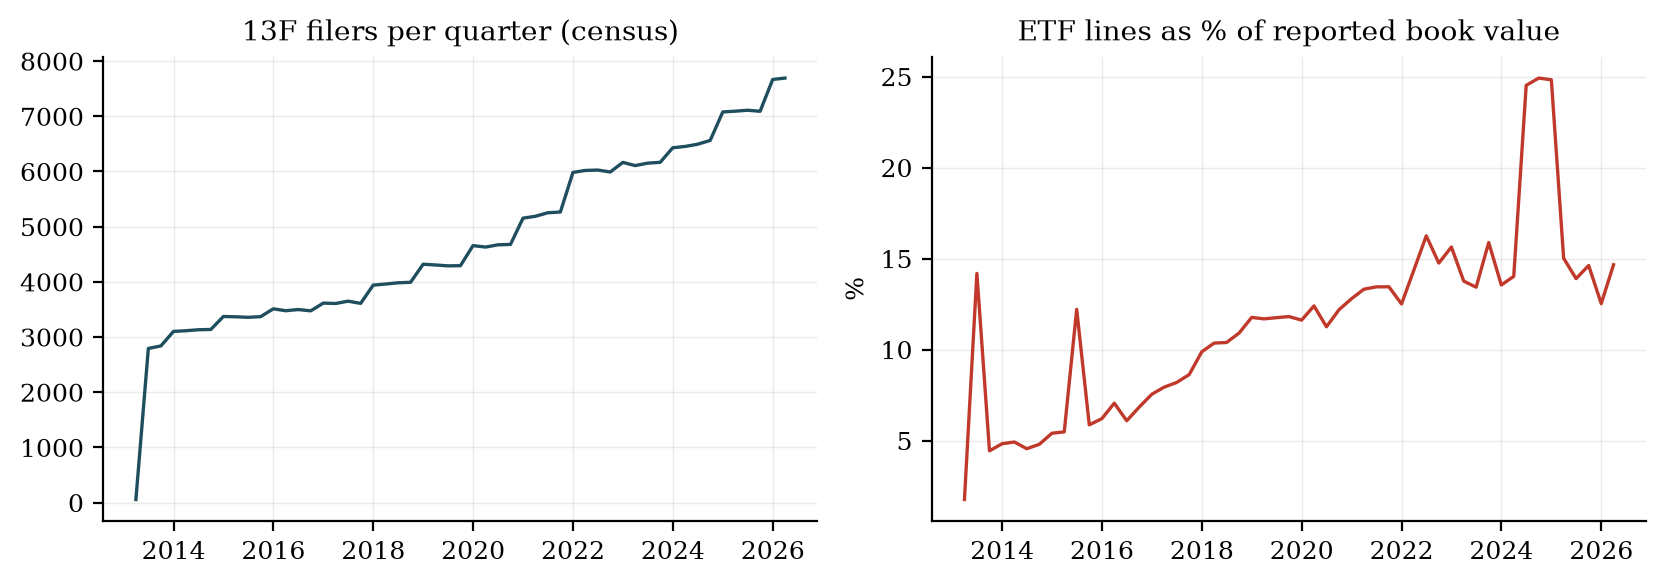
\includegraphics[width=.95\linewidth]{figs/f10_universe.png}
\caption{Left: 13F filers per quarter (census). Right: ETF lines as a
share of reported book value --- material and growing, and measured
to be innocuous for ranking signals (uniform, not differential,
contamination).}
\label{fig:universe}
\end{figure}

\paragraph{The ETF and passive-manager question.}
Because index products are 12--15\% of reported book value
(Figure~\ref{fig:universe}, right), we closed this question on three
independent fronts rather than by assumption. (i) \emph{Tradable
universe}: of 7{,}886 audited ETF instruments, one appears in the
crosswalk and none in the price panel --- ETFs were never buyable in
any backtest. (ii) \emph{Inside books}: purging ETF lines from filer
books changes the conviction threshold of $\sim$25\% of managers per
quarter and releases 17\% more conviction votes (single-stock bets
hidden behind index positions), yet the stock-level ranking is
unchanged (rank correlation $0.974$; top-100 overlap 97/100; paired
delta $+0.01\%$/quarter, $t=+0.08$): uniform contamination does not
distort a ranking signal. (iii) \emph{Passive managers as voters}:
only $\sim$10 filers per quarter have active share below 25\% --- the
giant index complexes, one third of aggregate AUM --- and they
produce $\sim$1\% of conviction votes; removing them moves the spread
by six basis points ($t=+1.19$). We summarize the asymmetry as
\emph{elephants without votes}: cutting active managers hurts,
cutting passive ones is noise, and the census stands on measured
parsimony.

\paragraph{Tradable asset universe.}
Common equities with a mapped current ticker and price
$\ge\$1$; no ADV floor at the signal-evaluation layer (the
illiquid short side is where several literature effects live), with
liquidity entering explicitly through each signal's denominator or
the engine's cost model rather than through silent universe
truncation. The production engine (Section~\ref{sec:engine}) applies
its own stricter tradability filter ($\$4$ price, $\$5$M median
dollar volume, 252 days of history).
